\subsection{L'interaction avec un examen}

Après avoir ouvert un examen, l'utilisateur se retrouve face à la fenêtre principale de l'application. Cette fenêtre présente la première tranche de l'examen ouvert. L'utilisateur peut la déplacer en utilisant l'écran tactile. Il peut aussi régler le niveau de zoom grâce au curseur prévu à cet effet. 
Le menu de l'application permet d'accéder aux informations de l'examen et de la coupe courante. Enfin, l'utilisateur peut basculer d'une coupe à une autre avec les boutons situés en haut de la fenêtre.\\

\begin{figure}[h]
\begin{center}
	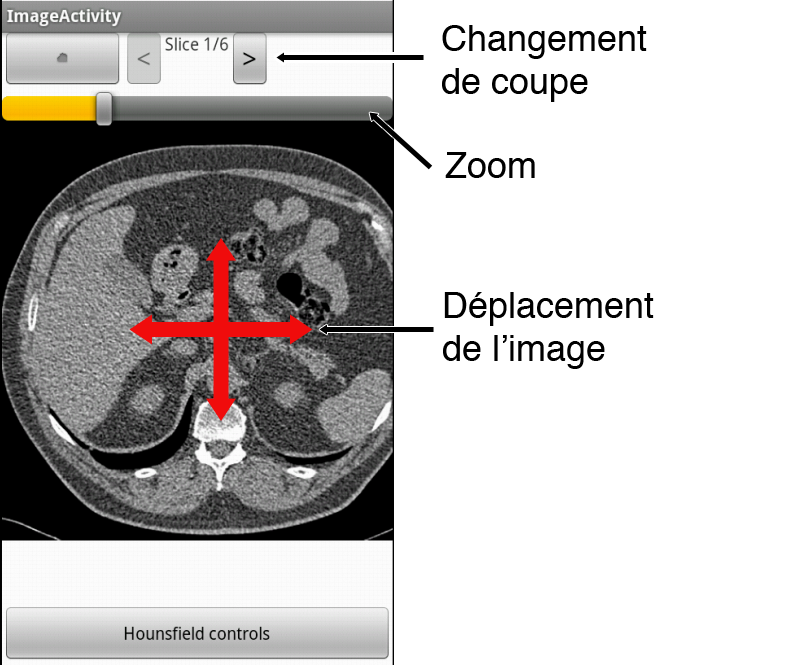
\includegraphics[width=11cm]{diams-capture-1.png}
\end{center}
	\caption{Fenêtre principale en mode déplacement}
\end{figure}

En bas de la fenêtre se trouve un menu coulissant permettant de gérer l'affichage de l'image à l'aide de l'échelle de Hounsfield. Deux curseurs permettent de régler la position et la taille de la fenêtre de valeurs à afficher. De plus, un menu déroulant permet de sélectionner des valeurs de contraste correspondant à des usages courants. L'affichage de l'image est alors mis à jour en temps réel.\\

L'utilisateur peut passer du mode déplacement de l'image au mode dessin sur le masque grâce à un bouton situé en haut de la fenêtre. Dans ce second mode, il est possible de réaliser des sélections de zone avec un crayon ou d'effacer des tracés existants. Une option permet de contrôler la largeur du tracé.\\

\begin{figure}[h]
\begin{center}
	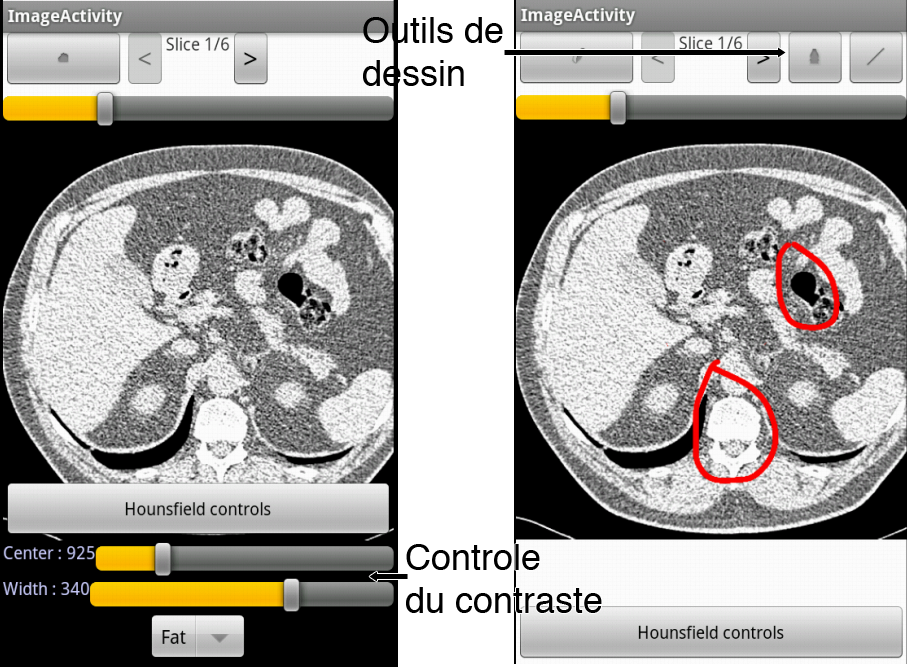
\includegraphics[width=11cm]{diams-capture-2.png}
\end{center}
	\caption{Réglages de contraste à gauche et mode dessin à droite}
\end{figure}
